\documentclass[10pt]{article}
\usepackage{fullpage}
\usepackage{graphicx}
%\usepackage{subfigure}
\usepackage{caption}
\usepackage{subcaption}
\usepackage{amsfonts,amsmath,amssymb,amsthm}

\theoremstyle{definition}
\newtheorem{definition}{Definition}[section]
\newtheorem{theorem}{Theorem}[section]

\begin{document}

\section{Gram Matrix}%
\label{sec:gram}
Our first attempt to analayse the SOM and spot potential differences between 
regular and random topologies has to do with the spectum of the Gram matrix 
defined by
%%
\begin{align}
    \label{eq:gram}
    {\bf M} &= {\bf Y}{\bf Y}^T \in \mathbb{R}^{m \times m},
\end{align}
%%
where $m$ is the number of neurons within the SOM and ${\bf Y} \in \mathbb{R}^{n \times m}$
is the SOM's activity matrix. The matrix ${\bf M}$ is called the Gram (or Grammian) 
matrix and in this case is nothing more than the data covariance matrix. The
distribution of its eigenvalues determine how much the input space has been
stretched or distorted. Skewed distributions suggest an anisotropy in the 
representations.

From a computational point of view we construct the ${\bf Y}$ matrix by
applying a set of stimuli ($50$ samples drawn from the input distribution) 
and we compute the activity of each neuron within the network. This means that
${\bf Y} \in \mathbb{R}^{m \times n}$, where $m=1024$ (the number of neurons)
and $n={2, 3}$ (two- or three-dimensional input samples). Then we use
equation~\eqref{eq:gram} to get the Gram (or the covariance) matrix. 

\section{Eigenvalues Distribution}%
\label{sec:dist}

To compute the eigenvalues distribution of the Gram matrix we sample
the activity of the neurons of each topology for $200$ different initial
conditions using $50$ input sample each time. 
At the end of sampling we get an \emph{ensemble} of $200$ Gram matrices
and we estimate the probability density by applying a Kernel Density Estimation
(KDE) on the eigenvalues of the ensemble. Finally, we quantify any differences
on the distributions of the regular and random SOMs by calculating the 
Wasserstein distance over two distributions (regular ($P$) and random ($Q$)).
The Wasserstein distance between two probability distributions $P$ and $Q$ is
given by
%%
\begin{align}
    W(P, Q) &= \inf_{\gamma \in \Pi(P, Q)}\{\mathbb{E}_{(x, y)\sim \gamma}\Big[||x -
    y||\Big]\},
\end{align}
%%
where $\Pi(P, Q)$ denotes the set of all joint distributions $\gamma (x, y)$, 
whose marginals are $P$ and $Q$, respectively. Intuitively, $\gamma (x,y)$
indicates  how  much ``mass'' must be transported from $x$ to $y$ to transform
the distribution $P$ into the distribution $Q$. 

\subsection{Experiment 1}
The first experiment shows how a two-dimensional SOM maps a one-dimensional
uniform distribution ($x_i \sim \mathcal{U}(0, 1)$, where $x_i$ is the $i$-th
input sample). After we obtain the Kohonen and Voronoi SOM codebooks we
estimate the eigenvalues distribution of the corresponding Gram matrices (see
Section~\ref{sec:gram} on how to construct the Gram matrix) using the sampling
method described in~\ref{sec:dist}. Figure~\ref{Fig:distributions}{\bfseries
\sffamily A} shows the distributions of the eigenvalues for both cases, regular
(blue) and random (black). The Wasserstein distance is given at the title of
the panel.

\subsection{Experiment 2a}
In this experiment we replace the one-dimensional distribution with a
two-dimensional uniform distribution of an annulus. The rest of the analysis 
remains the same as in Experiment $1$ and the results are shown in
Figure~\ref{Fig:distributions}{\bfseries \sffamily B}.

\subsection{Experiment 2b}
In this experiment we replace the one-dimensional distribution with a
two-dimensional uniform distribution of an annulus. The rest of the analysis 
remains the same as in Experiment $1$ and the results are shown in
Figure~\ref{Fig:distributions}{\bfseries \sffamily C}.

\subsection{Experiment 3}
In the last experiment, we tested both the Kohonen and the VSOM algorithms 
on mapping a three-dimensional uniform distribution (cube). 
Figure~\ref{Fig:distributions}{\bfseries \sffamily} illustrates the 
distributions of eigenvalues for both algorithms.


\begin{figure}[!htpb]
     \centering
     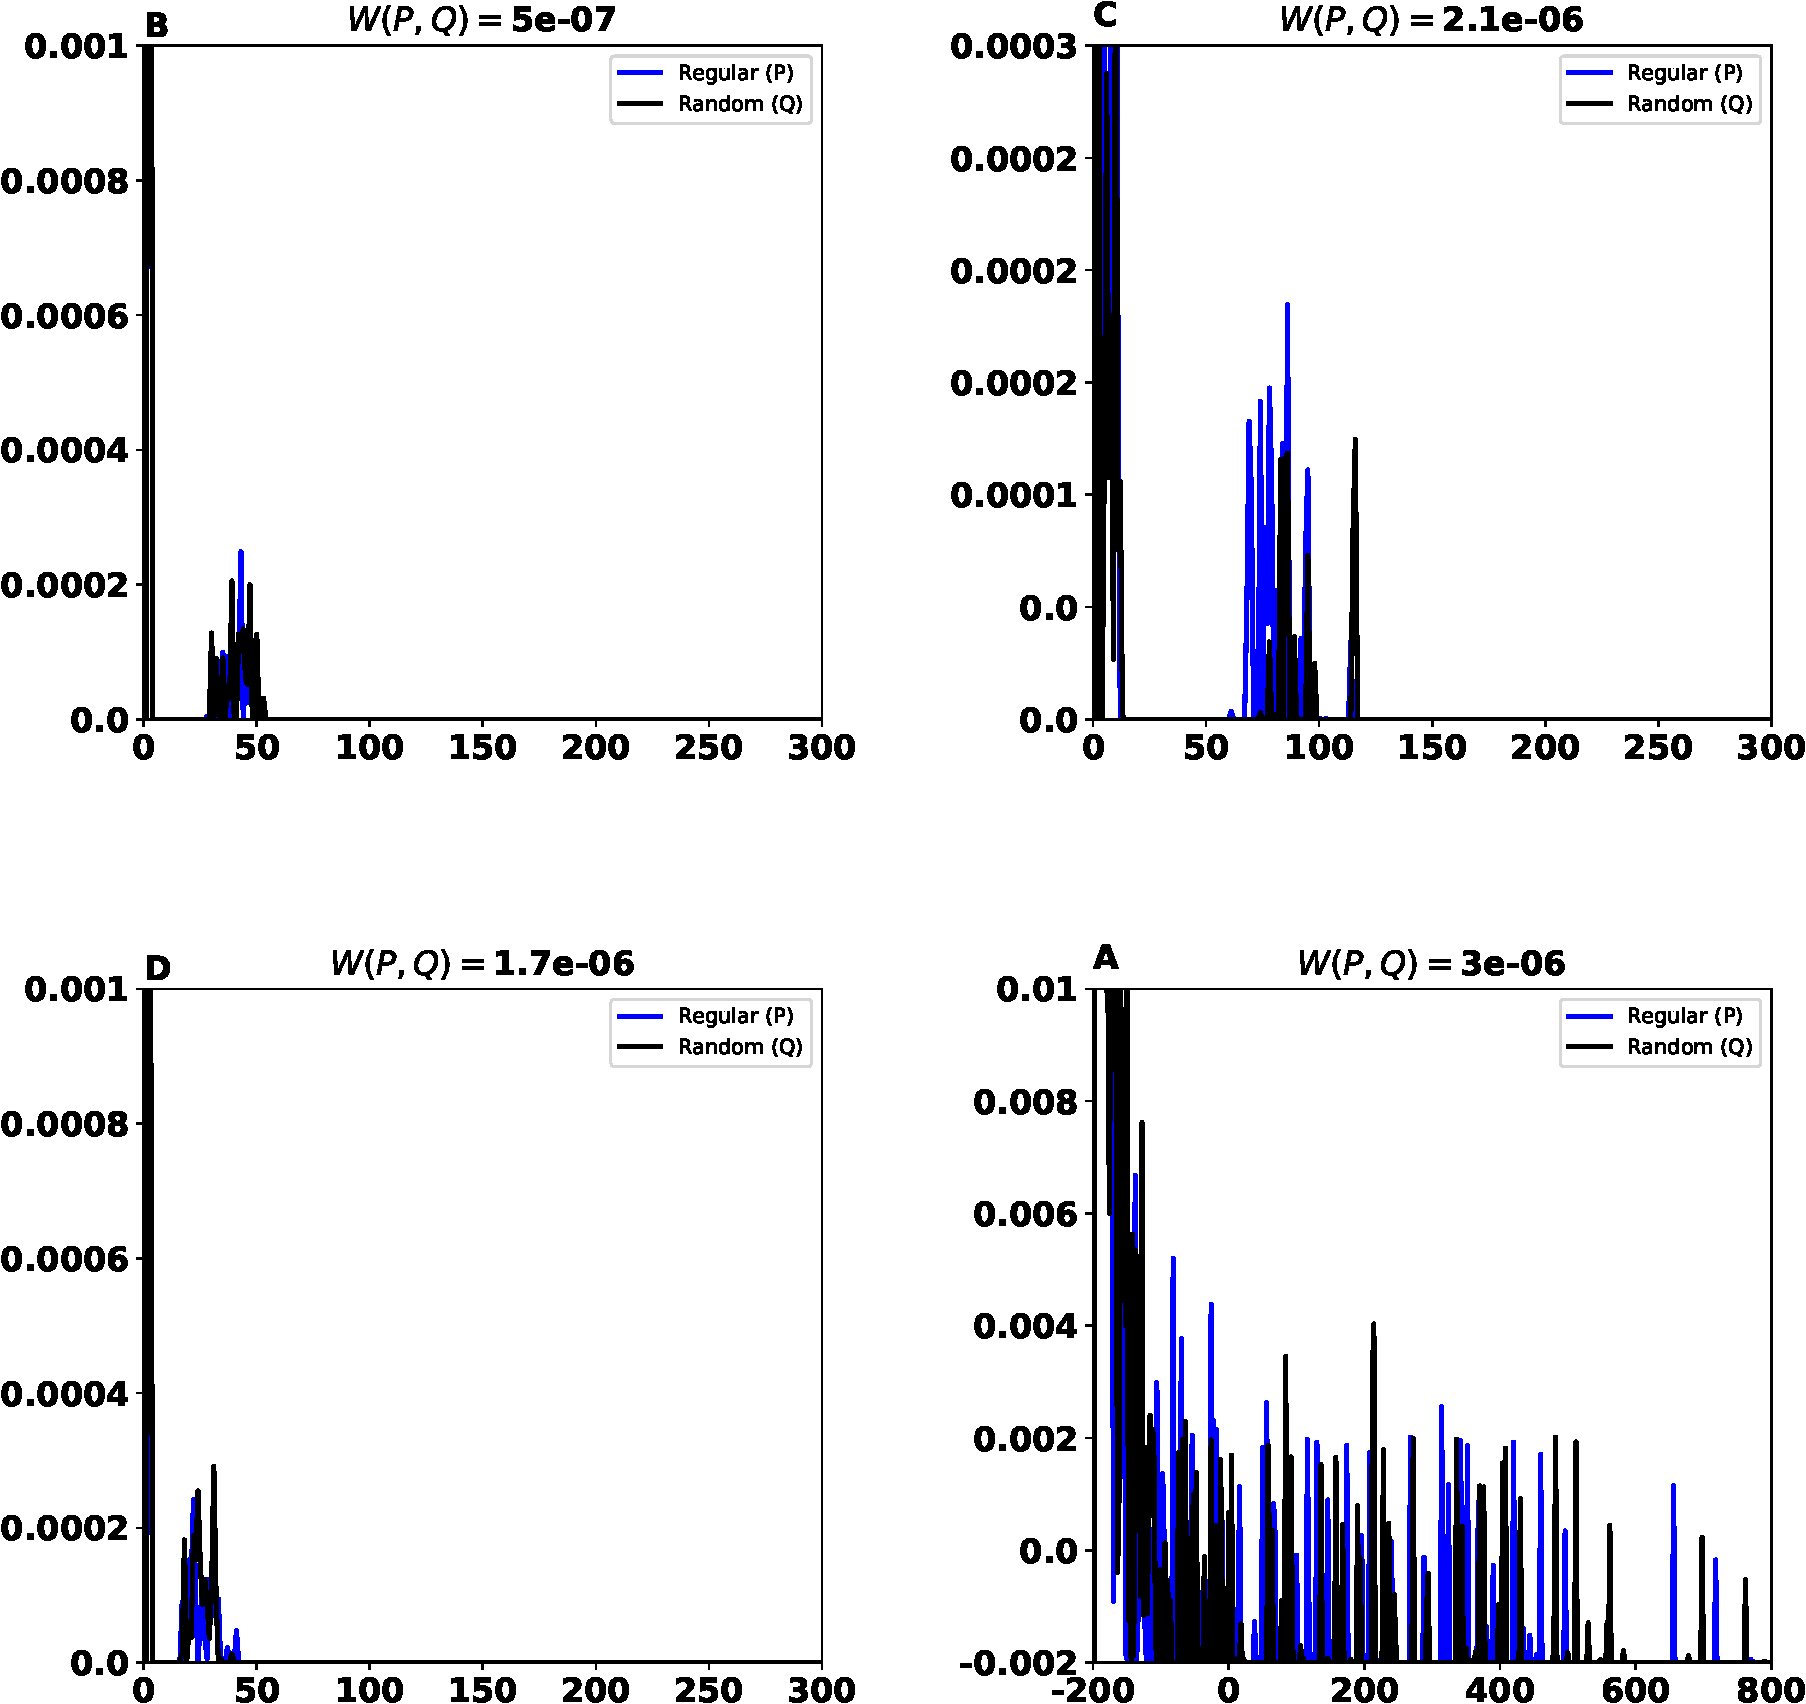
\includegraphics[width=\textwidth]{./figures/eig-distributions.pdf}
     \caption{{\bfseries \sffamily Eigenvalues Distributions}
     {\bfseries \sffamily A} Experiment $1$, a two-dimensional SOM
     maps a one-dimensional uniform distribution of $[0, 1]$.
     {\bfseries \sffamily B} Experiment $2$a a two-dimensional uniform
     distribution of an annulus is being mapped by a two-dimensional SOM\@.
     {\bfseries \sffamily C} Experiment $2$b a two-dimensional uniform
     distribution with holes is the input space for a two-dimensional SOM\@. 
     {\bfseries \sffamily D} Experiment $3$ A two-dimensional SOM learns the
     representations of a three-dimensional uniform distribution (cube). In 
     all the panels blue color indicates the standard Kohonen SOM and the 
     black color shows the VSOM.}%
     \label{Fig:distributions}
\end{figure}

%\section*{Pseudospectra Analysis}

%Another way to unveil and understand the properties of the SOMs with both 
%regular and random topologies is the pseudospectra analysis. First we give 
%the definitions of pseudospectra. 

%Let ${\bf V} \in \mathbb{R}^{m \times n}$ be a rectangular matrix, not
%necessarily normal (\emph{i.e.}, ${\bf V}{\bf V}^{*} \neq {\bf V}^{*}{\bf V}$).
%The $\epsilon$-pseudospectra ($\Lambda_{\epsilon}$) is the set of 
%$\epsilon$-eigenvalues, a closed subset of $\mathbb{C}$.
%%%
%\begin{definition}[$\epsilon$-Pseudospectra]
%	\label{def:psd1}
%    Let ${\bf V} \in \mathbb{C} \text{ or } \mathbb{R}$, 
%    $z \in \mathbb{C}$ and $\tilde{{\bf I}} \in \mathbb{R}^{m \times n}$ (the identity 
%    matrix with ones on the main diagonal and zeros elsewhere), then the $\epsilon$-pseudospectra
%    $\Lambda_{\epsilon} = \{z \in \mathbb{C}: ||({\bf V} - z\tilde{{\bf I}}){\pmb \upsilon}||\leq \epsilon
%    \text{ for some } \pmb{\upsilon} \in \mathbb{C}^n, ||\pmb{\upsilon}|| = 1\}$.
%\end{definition}
%%%
%%%
%\begin{definition}[$\epsilon$-Pseudospectra]
%	\label{def:psd2}
%    Let ${\bf V} \in \mathbb{C} \text{ or } \mathbb{R}$, 
%    $z \in \mathbb{C}$ and $\tilde{{\bf I}} \in \mathbb{R}^{m \times n}$ (the identity 
%    matrix with ones on the main diagonal and zeros elsewhere), then the $\epsilon$-pseudospectra
%    $\Lambda_{\epsilon} = \{z \in \mathbb{C}: \sigma_{\min}(z\tilde{{\bf I}}-{\bf V})\leq \epsilon \}$.
%\end{definition}
%%%
%Definitions~\ref{def:psd1} and~\ref{def:psd2} are equivalent, and both 
%account for the computation of $\Lambda_{\epsilon}$ of rectangular matrices of dimension
%$m \times n$, where $m \geq n$. In this work we apply the pseudospectra 
%analysis on the Gram matrix given by~\eqref{eq:gram}. 
%The results from the pseudospectra analysis are shown in Figure~\ref{Fig:psas}. 


% \begin{figure}[!htpb]
%      \begin{subfigure}{0.5\textwidth}
%          \centering
%          \includegraphics[width=.8\textwidth]{./data/experiment-1-psa.pdf}
%          \caption{Experiment $1$--$1$D uniform distribution.}%
%          \label{Fig:psa_exp1}
%      \end{subfigure}
%      % \hfill
%      \begin{subfigure}{0.5\textwidth}
%          \centering
%          \includegraphics[width=.8\textwidth]{./data/experiment-2-psa.pdf}
%          \caption{Experiment $2$a--$2$D uniform distribution (annulus).}%
%          \label{Fig:psa_exp2a}
%      \end{subfigure}
%      \newline 
%      \begin{subfigure}{0.5\textwidth}
%          \centering
%          \includegraphics[width=.8\textwidth]{./data/experiment-2-bis-psa.pdf}
%          \caption{Experiment $2$b--$2$D uniform distribution with holes.}%
%          \label{Fig:psa_exp2b}
%      \end{subfigure}
%      \begin{subfigure}{0.5\textwidth}
%          \centering
%          \includegraphics[width=.8\textwidth]{./data/experiment-3-psa.pdf}
%          \caption{Experiment $3$--$3$D uniform distribution (cube)}%
%          \label{Fig:psa_exp3}
%      \end{subfigure}
%     \caption{Pseudospectra of Gram matrix for experiments $1$, $2$, and $3$.
%     Panels on the left side show the Pseudospectra for the Kohonen's SOM map
%     and on the right side are the Pseudospectra of the VSOM map.}%
%     \label{Fig:psas}
% \end{figure}

\noindent \rule{\textwidth}{1pt}

\section{Topological Data Analysis}

A different approach for analyzing the SOMs comes from the field of Toplogical
Data Analysis (TDA). TDA is a field of applied mathematics that provides 
means to study topological structures of data sets (particularly cloud points
with no apparent structure). TDA tools are insensitive to dimension reduction
and noise that has contaminate the data. 
Many tools belong to the general field of TDA, however in this work we are
going to focus on the persistence homology. 

What we would like to achieve using TDA is to identify topological differences 
between neural spaces of different neural manifolds provided by different
SOM algorithms. Unfortunately, the exact manifold (or distribution) of the
input space is not known and the SOM algorithms only approximate it. So one 
way to overcome this problem is to approximate the input and neural manifolds
using simpler spaces. Of course, this kind of spaces should respect the
topological structure of the original manifolds. Such kind of spaces are the
simplicial complexes. A simplicial complex is a space that has been constructed
out of intervals, triangles, and other higher dimensional simplices. To start
approximating the input and neural manifolds we define a family of thresholds
$\alpha$ (or radius) such that for every such $\alpha$ we center a ball of
radius $\alpha$ on each data point and look for intersections of those balls.
For instance, if $\alpha$ is too small then there are no intersecting balls 
(disjoint set of balls). On the other hand, if $\alpha$ is too large then 
a single connected blob emerges. As $\alpha$ varies from a low to a large 
value holes open and close as different balls start intersecting as they 
get inflated. Hence, topological relevant information is being revealed as 
the process of inflating balls continuous. The radius of the balls,
$\alpha$, is called the ``persistence'' parameter and the previously described 
process of inflating balls around our data point builds a diagram 
called ``persistence'' diagram (and the persistence barcode). 
We focus our analysis more on the two first homology groups, which are:
$H_0$, which describes the path-connected components of a topological space 
$\mathcal{X}$ (homeomorphic to a point), and $H_1$ that defines the 
one-dimensional holes (homeomorphic to circle).

Persistence indicates which topological features (holes) persist more as 
we vary the persistence parameter $\alpha$ (radius). Features that last long
enough (they persist under many increases of the parameter $\alpha$) are
considered to be significant. In this work we drop the mathematical definitions
since they are out of context and we only use the persistent diagrams for 
analyzing our results (we refer the reader
to~\cite{chazal:2017,ghrist:2008,zomorodian:2005} for a rigorous mathematical
introduction to Topological Data Analysis). For our analysis we use the Python
programming language and the Gudhi library~\cite{maria:2014}.

\begin{figure}[!htpb]
     \centering
     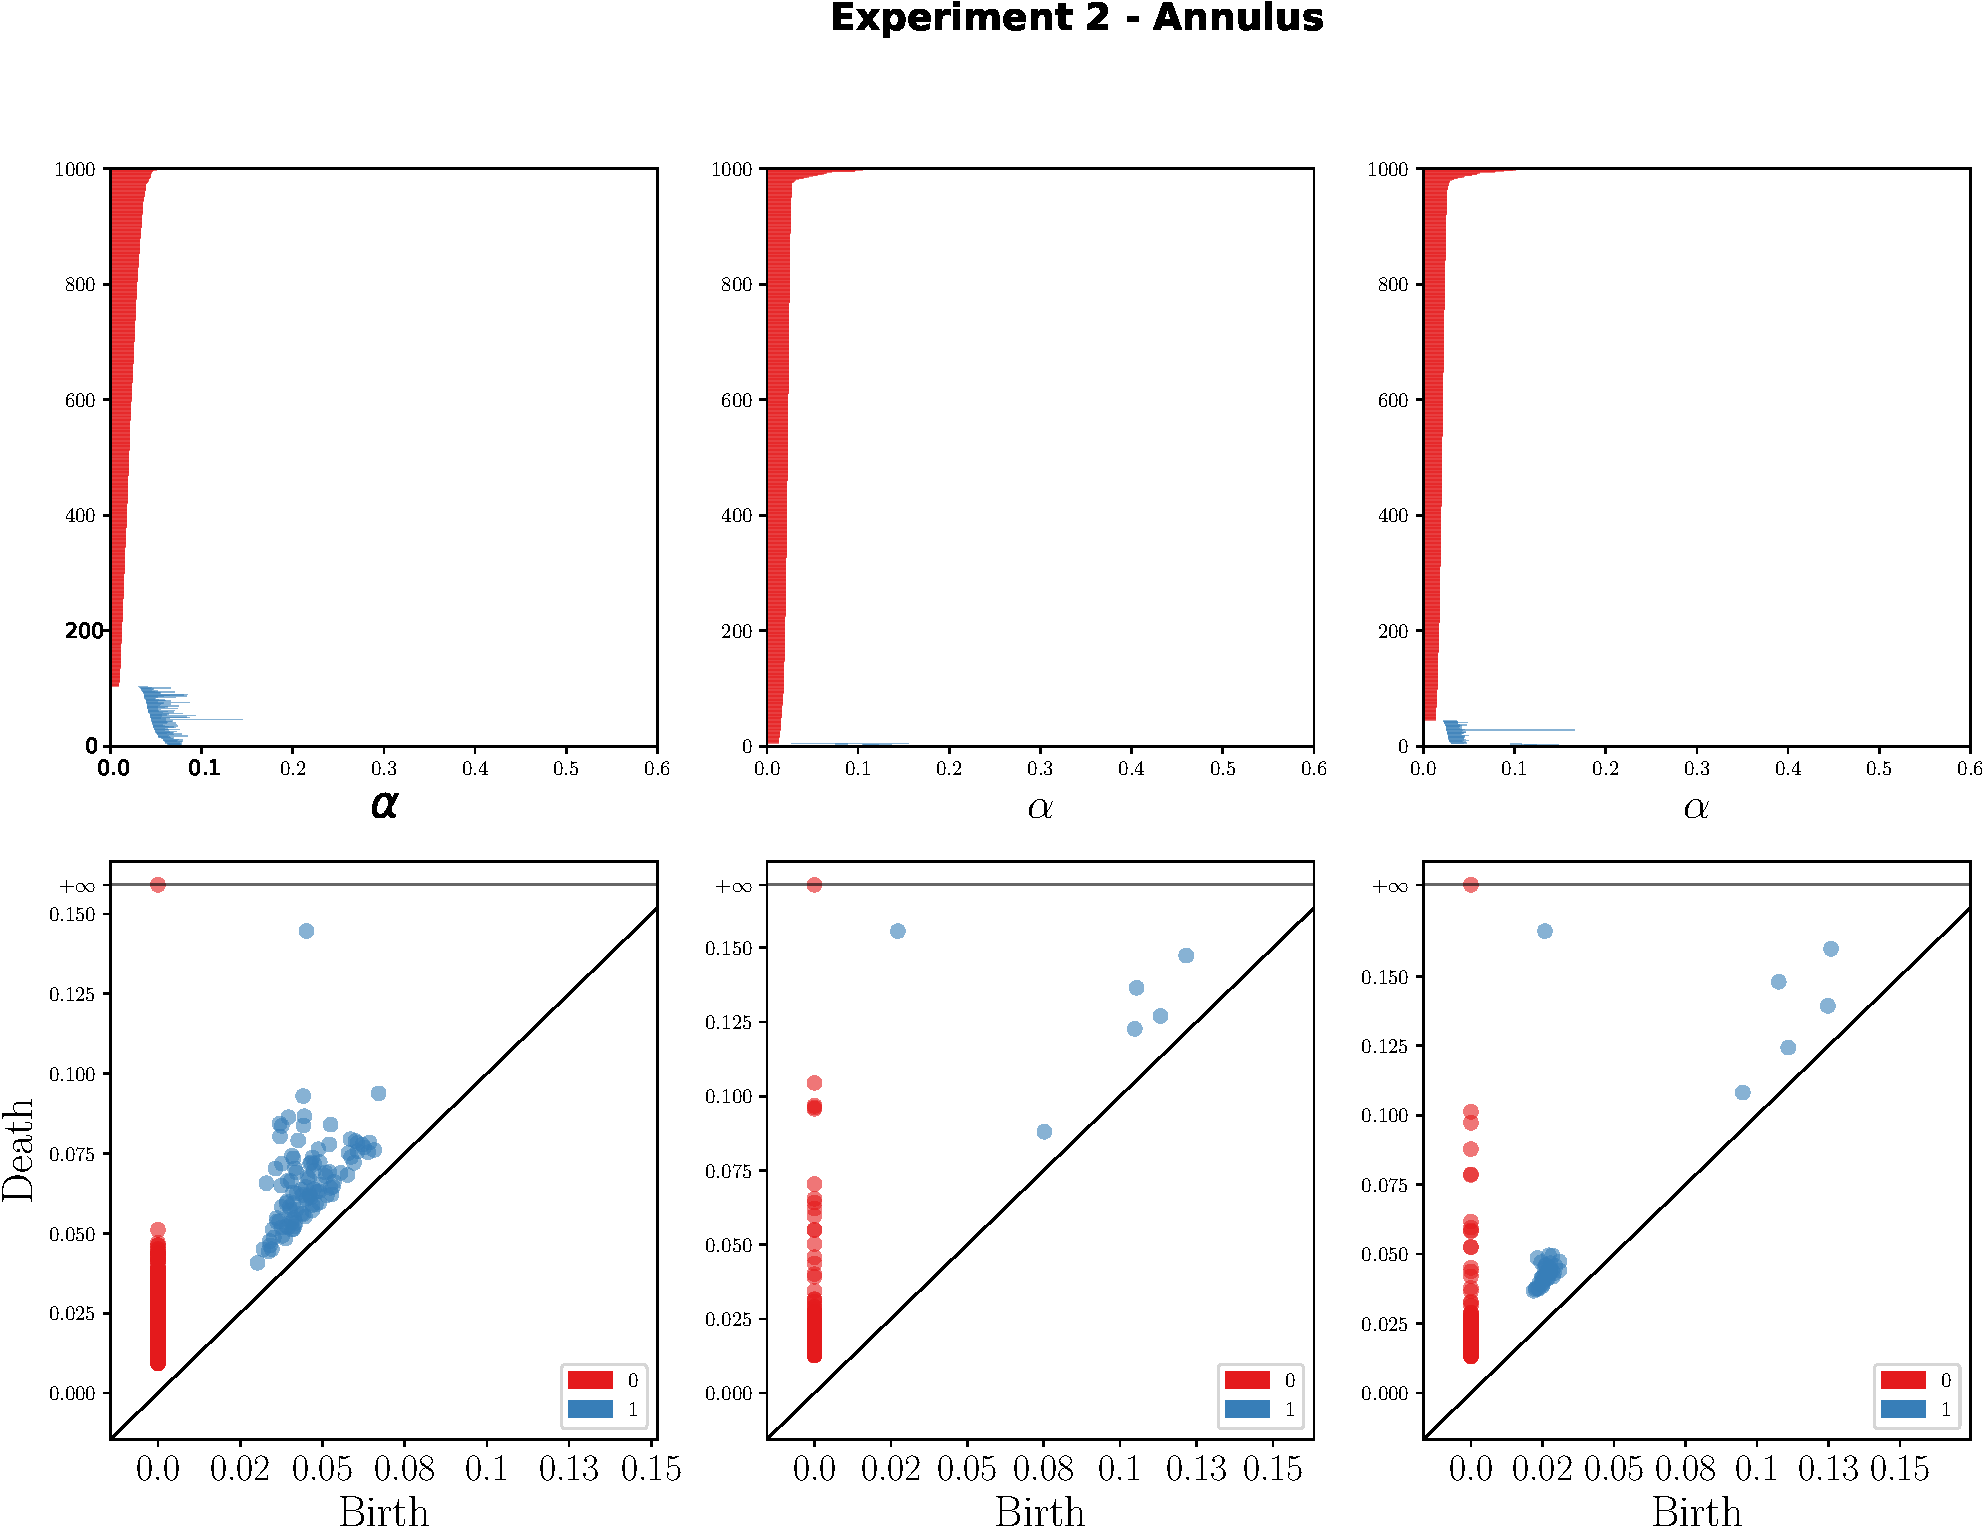
\includegraphics[width=\textwidth]{./figures/experiment-2-pd.pdf}
     \caption{Experiment $2$--$2$D uniform annulus.}%
     \label{Fig:persistence_exp2}
\end{figure}

\begin{figure}[!htpb]
     \centering
     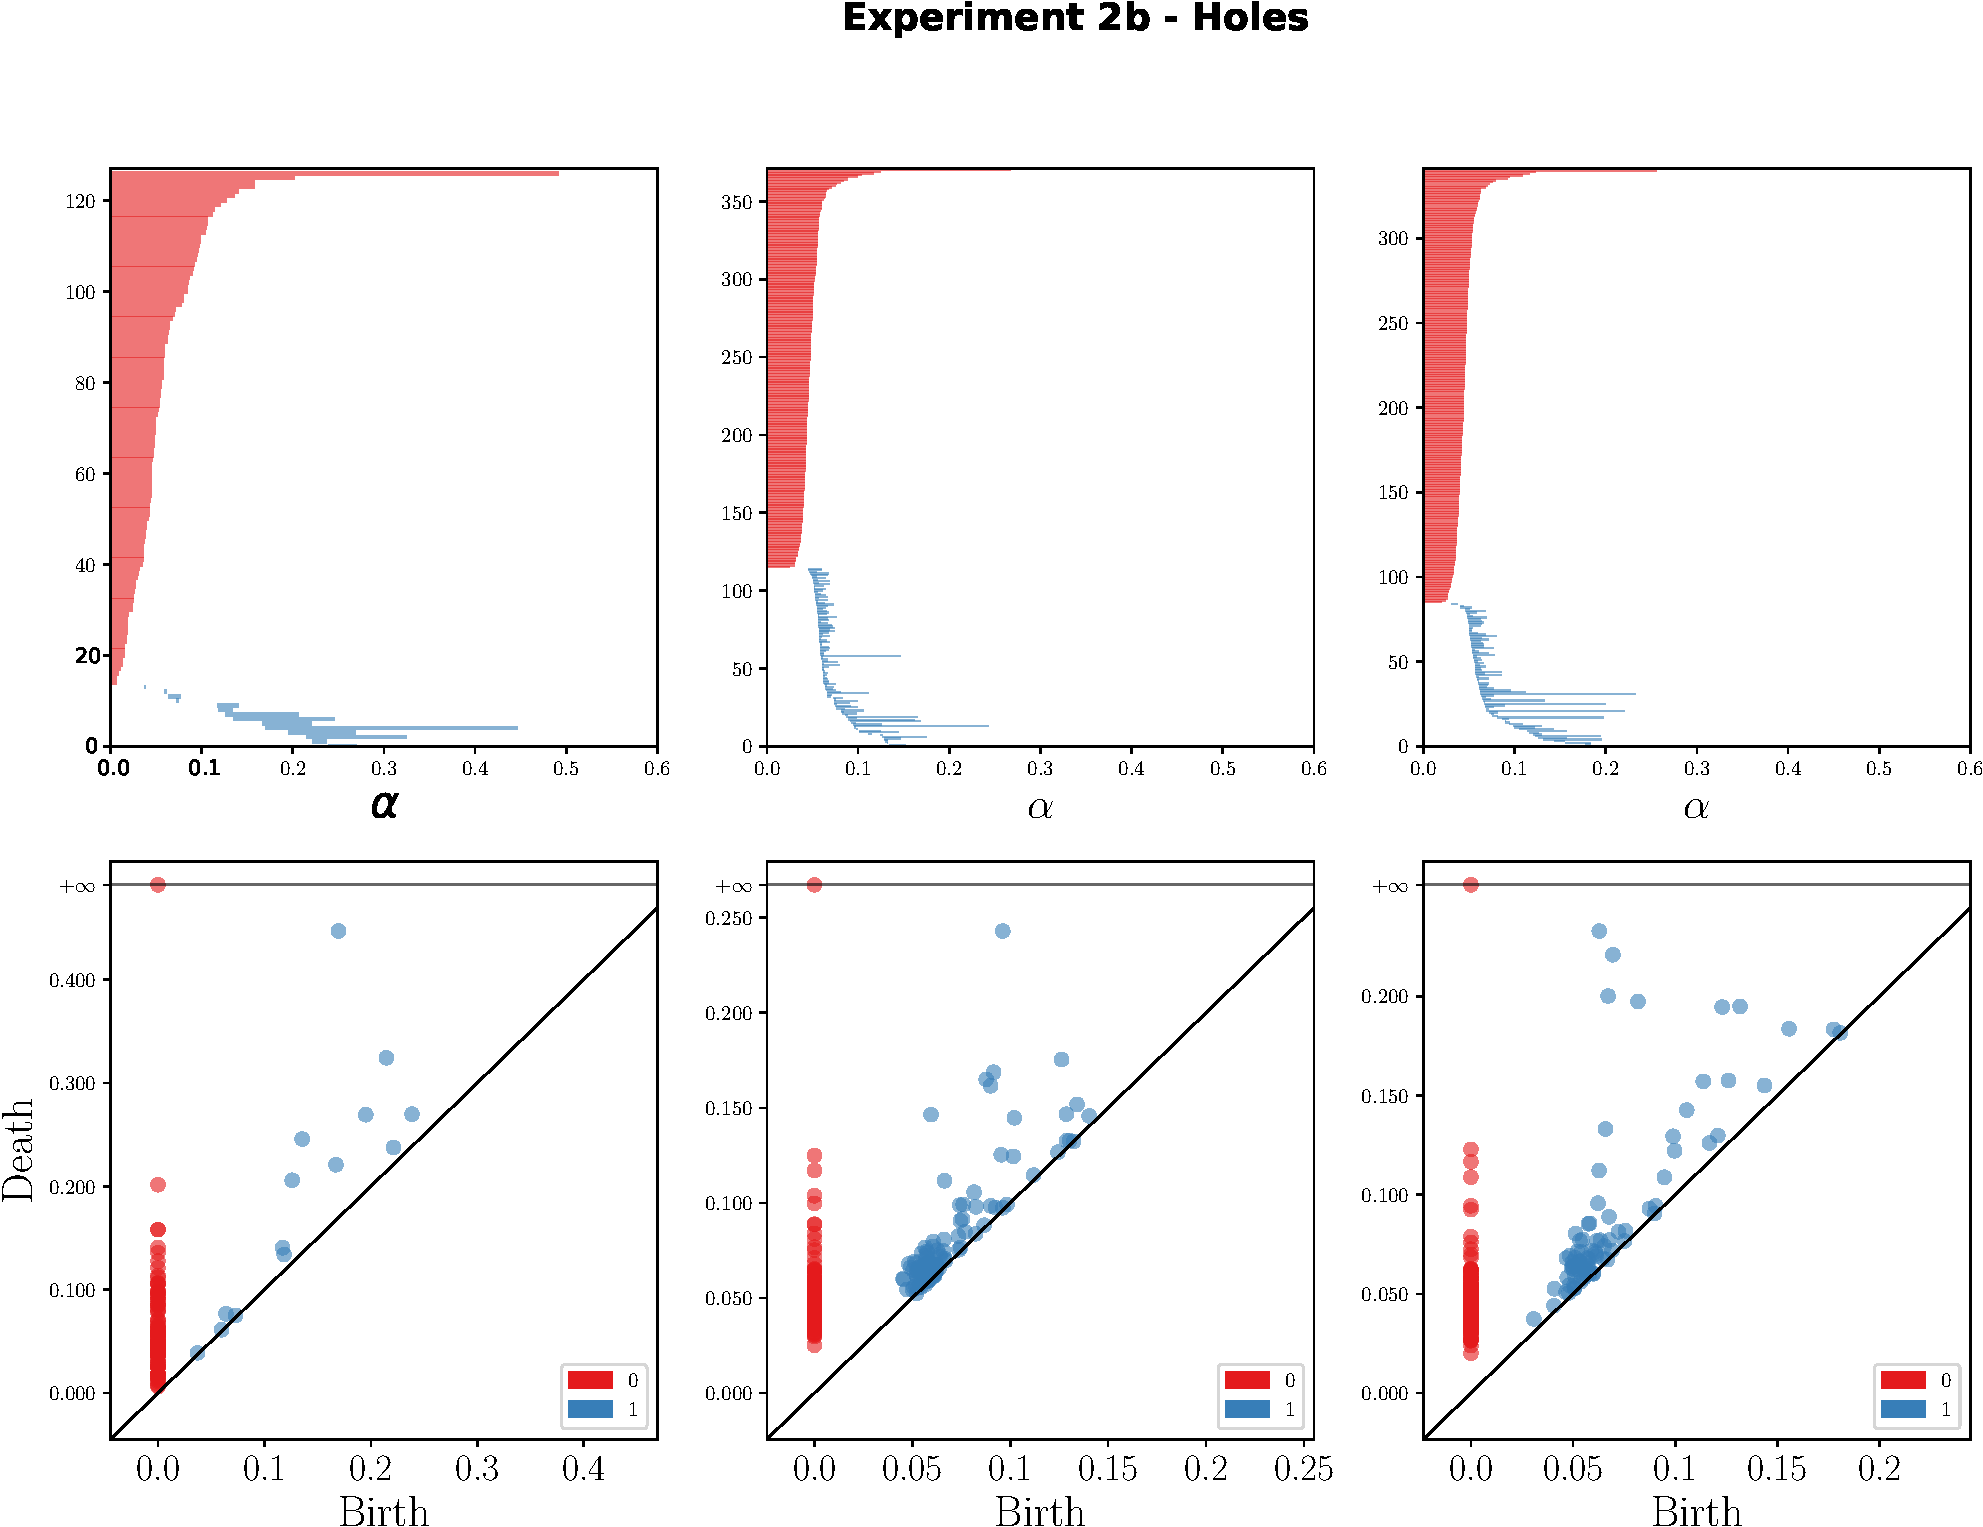
\includegraphics[width=\textwidth]{./figures/experiment-2-bis-pd.pdf}
     \caption{Experiment $2$--$2$D random distribution with holes.}%
     \label{Fig:persistence_exp2b}
\end{figure}

\bibliographystyle{apalike}
\bibliography{biblio}

\end{document}
